\documentclass[11pt]{article}
\usepackage[margin=1in]{geometry} 
\usepackage{amsmath,amsthm,amssymb,amsfonts}
\usepackage{listings}
\usepackage{graphicx}
\usepackage{lipsum,calc}
\usepackage[shortlabels]{enumitem}
 
\newcommand{\N}{\mathbb{N}}
\newcommand{\Z}{\mathbb{Z}}

\newenvironment{problem}[2][Problem]{\begin{trivlist}
\item[\hskip \labelsep {\bfseries #1}\hskip \labelsep {\bfseries #2.}]}{\end{trivlist}}

\begin{document}
\title{CSE 574 Homework 2}
\author{Zackary Crosley}
\maketitle

\begin{problem}{1}
	Uninformed Search - Iterative Leng
	\begin{enumerate}
		\item Show this algorithm is optimal for general path costs.
		
		\begin{verse}
			Suppose, to the contrary iterative lengthening selects a suboptimal route. That is for an optimal path A, A has a unit length less than or equal to all other possible paths. Suboptimal path B has unit length larger than A. Selecting B would require it to be seen before or in the same iteration as A. However, since iterative lengthening increases path length by a unit value each time A would have been encountered in an iteration before B and thus B wouldn't have been selected. Therefore, this algorithm must be optimal.
		\end{verse}
		\item Consider a uniform tree with branching factor b, solution depth d, and unit cost. How many iterations will iterative lengthening require?
		\begin{verse}
			Since the paths are all unit cost, the number of iterations of the iterative lengthening algorithm would be equal to the unit cost of the most optimal path to the solution. Since each successive layer of depth in the tree is one greater path cost, this is equivalent to the solution depth d.
		\end{verse}
		\item Now consider step costs drawn from the continuous range [$\epsilon$, 1], where $0 < \epsilon < 1$. How many iterations are required in the worst case?
		\begin{verse}
			Since the cost is continuous it is possible for the search to take considerably longer. If you imagine a tree that is non-finite and has a never ending path leading away from the solution with path increments of exactly $\epsilon$, then the tree will take $\frac{n}{\epsilon}$ iterations where n is the optimal cost to reach the solution. This is because the iteration will step up the path cost by exactly $\epsilon$ each iteration. The path cost to reach the solution would be $d\epsilon \leq cost \leq d$ since the path cost is in range [$\epsilon$, 1]. In the worst case, where the cost is d, this would result in a total number of iterations $\frac{d}{\epsilon}$
		\end{verse}
	\end{enumerate}
\end{problem}
\begin{problem}{2}
Apply the A* search on this graph to reach Bucharest from Lugoj using the straight-line distance heuristic function. Show the sequences of nodes which are considered by the algorithm. Show the f,g,and h for each node.
\begin{verse}
	Search Process by Phase
\end{verse}
\begin{enumerate}[label={Phase \Roman*},leftmargin=1.25in]
	\item [Phase 1] From Lugoj
		\begin{verse}
			Mehadia h(n) = 241, g(n) = 70, f(n) = 311
			Timisoara h(n) = 329, g(n) = 111, f(n) = 440
		\end{verse}
	\item [Phase 2] From Mehadia
		\begin{verse}
			Dobreta h(n) = 242, g(n) = 145, f(n) = 387
		\end{verse}
	\item [Phase 3] From Dobreta
		\begin{verse}
			Craiova h(n) = 160, g(n) = 265, f(n) = 425
		\end{verse}
	\item [Phase 4] From Craiova
		\begin{verse}
			Rimnicu Vilcea h(n) = 193, g(n) = 411, f(n) = 604
			Pitesti h(n) = 100, g(n) = 403, f(n) = 503
		\end{verse}
	\item [Phase 5] From Timisoara
		\begin{verse}
			Arad h(n) = 366, g(n) = 229, f(n) = 595
		\end{verse}
	\item [Phase 6] From Pitesti
		\begin{verse}
			Bucharest h(n) = 0, g(n) = 504, f(n) = 504
		\end{verse}
\end{enumerate}
\end{problem}
\begin{problem}{3}
Heuristic Properties
\begin{enumerate}
	\item Is h(n) admissable?
	\begin{verse}
		No. Admissability requires that for every point in the graph h(n) overestimates the distance to the goal. In this case, our goal is G. At point A the heuristic provides an estimate distance of 1, but the actual distance is 4. Therefore the heuristic cannot be admissable.
	\end{verse}
	\item Is h(n) consistent?
	\begin{verse}
		No. Consistency (monotonicity) requires that for any node n and an arbitrary successor n' the heuristic estimation for n cannot exceed the actual cost of reaching n' plus the heuristic estimation for n'. If we look at nodes S and A, the heuristic evaluation of S is 7. However, the actual cost to A is 4 and A has a heuristic cost of 1, for a total of 5. Since 5 < 7, this is not a consistent heuristic.
	\end{verse}
	\item Show A* using GRAPH-SEARCH on the provided state space returns a suboptimal solution.
	\begin{enumerate}[label={Phase \Roman*},leftmargin=1.25in]
		\item [Phase 1] From S
			\begin{verse}
				B h(n) = 5, g(n) = 2, f(n) = 7
				A h(n) = 1, g(n) = 4, f(n) = 5
			\end{verse}
		\item [Phase 2] From A
			\begin{verse}
				G h(n) = 0, g(n) = 8, f(n) = 8
			\end{verse}
	\end{enumerate}
	\begin{verse}
		This totally misses the possible route S -> B -> A -> G which has a path cost of 7. A* will not find alternative routes once the destination is reached. Therefore this search will return a suboptimal result.
	\end{verse}
\end{enumerate}
\end{problem}
\begin{problem}{4}
	\begin{figure}
		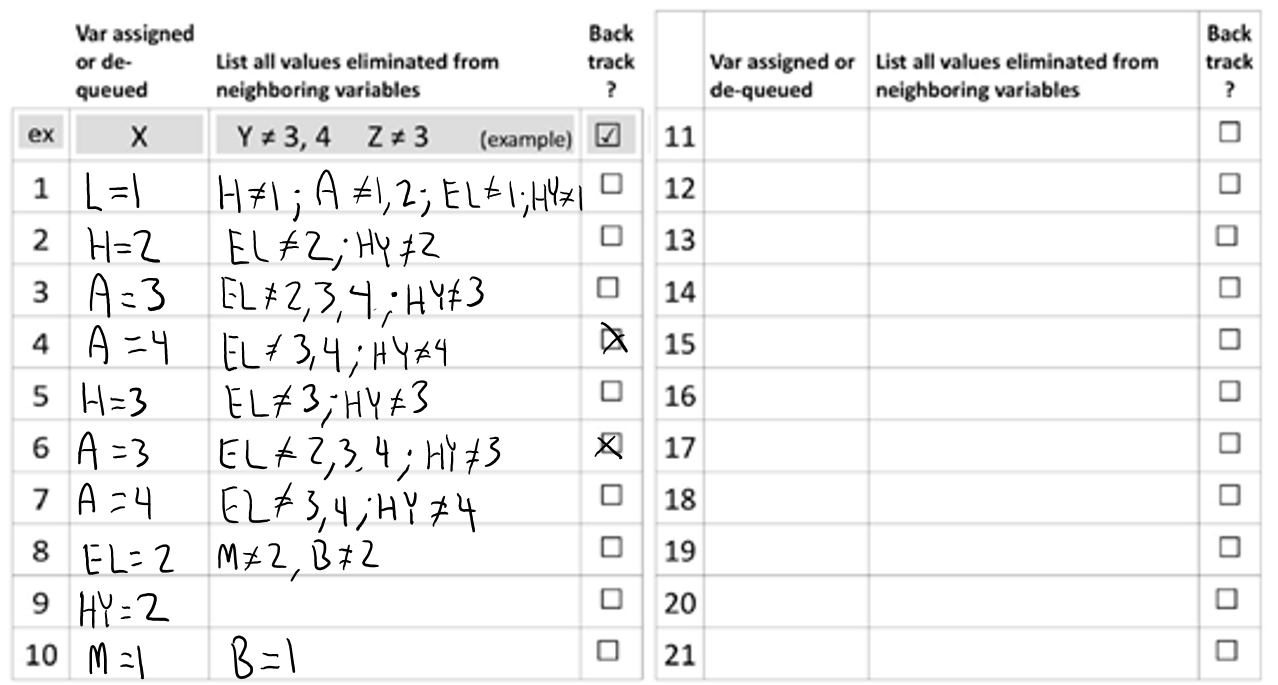
\includegraphics[scale=1]{cse545_hw2_p4_1.PNG}
		\caption{Problem 4 Constraint Satisfaction Search Table.}
		\label{fig.bfs}
	\end{figure}
	\begin{figure}
		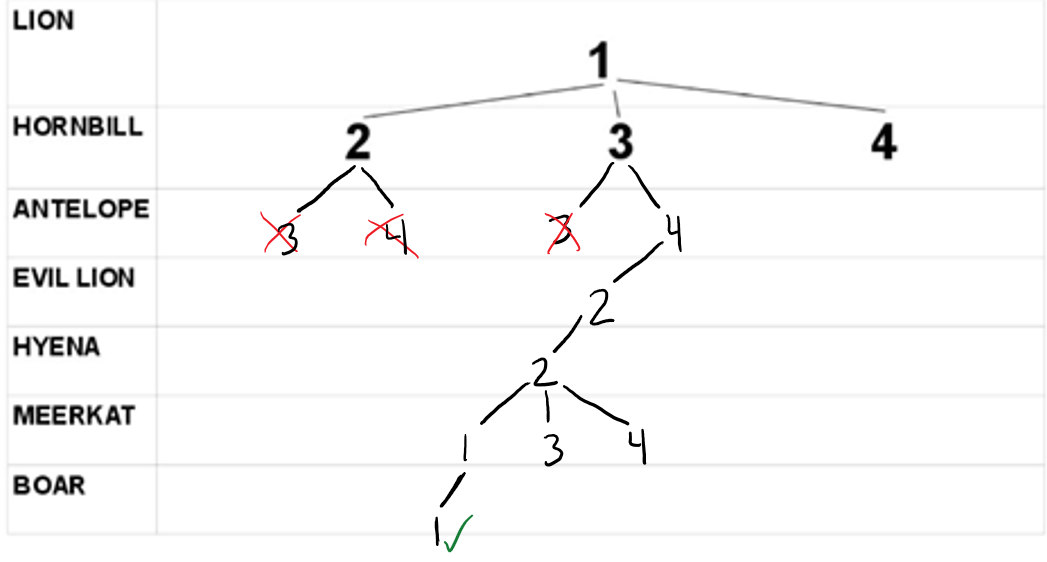
\includegraphics[scale=1]{cse545_hw2_p4_2.PNG}
		\caption{Problem 4 Constraint Satisfaction Search Tree.}
		\label{fig.bfs}
	\end{figure}
	\begin{verse}
		See Figure 1 and 2.
	\end{verse}
\end{problem}
\begin{problem}{5}
	\begin{figure}
		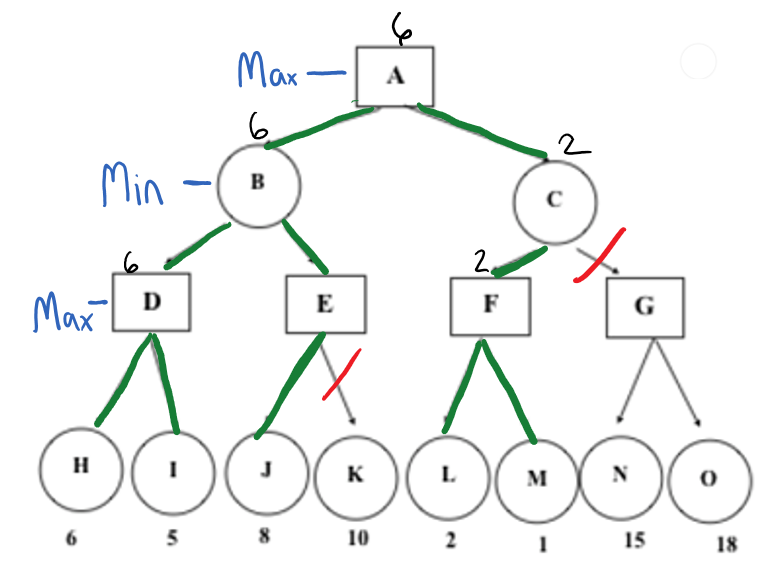
\includegraphics[scale=1]{cse545_hw2_p5.PNG}
		\caption{Problem 5 Alpha-Beta Pruning.}
		\label{fig.bfs}
	\end{figure}
	\begin{verse}
		See Figure 3.
	\end{verse}
\end{problem}
\begin{problem}{6} Adversarial Search
\begin{enumerate}
	\item Draw the complete game tree.
		\begin{figure}
			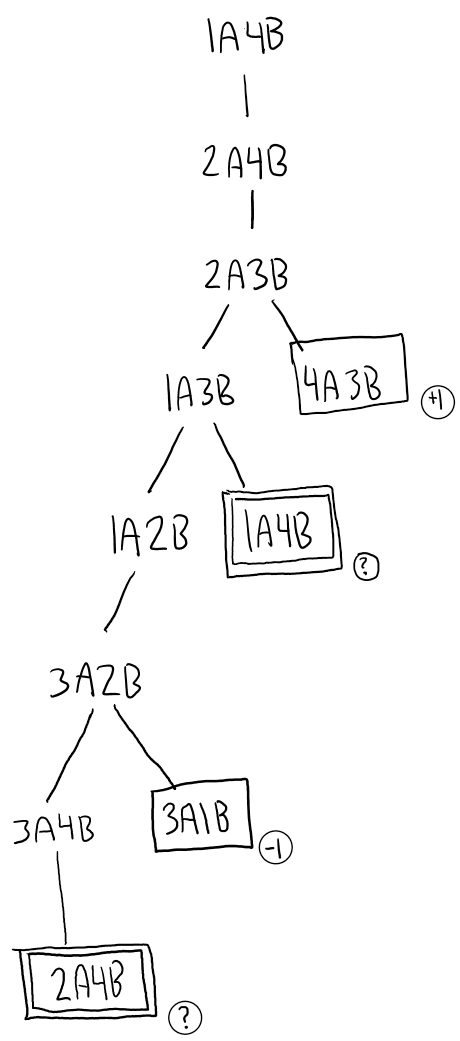
\includegraphics[scale=1]{cse545_hw2_p6_a.PNG}
			\caption{Problem 6a Adversarial Game Tree.}
			\label{fig.bfs}
		\end{figure}
		\begin{verse}
			See Figure 4.
		\end{verse}
	\item Mark each node with their minimax values.
		\begin{figure}
			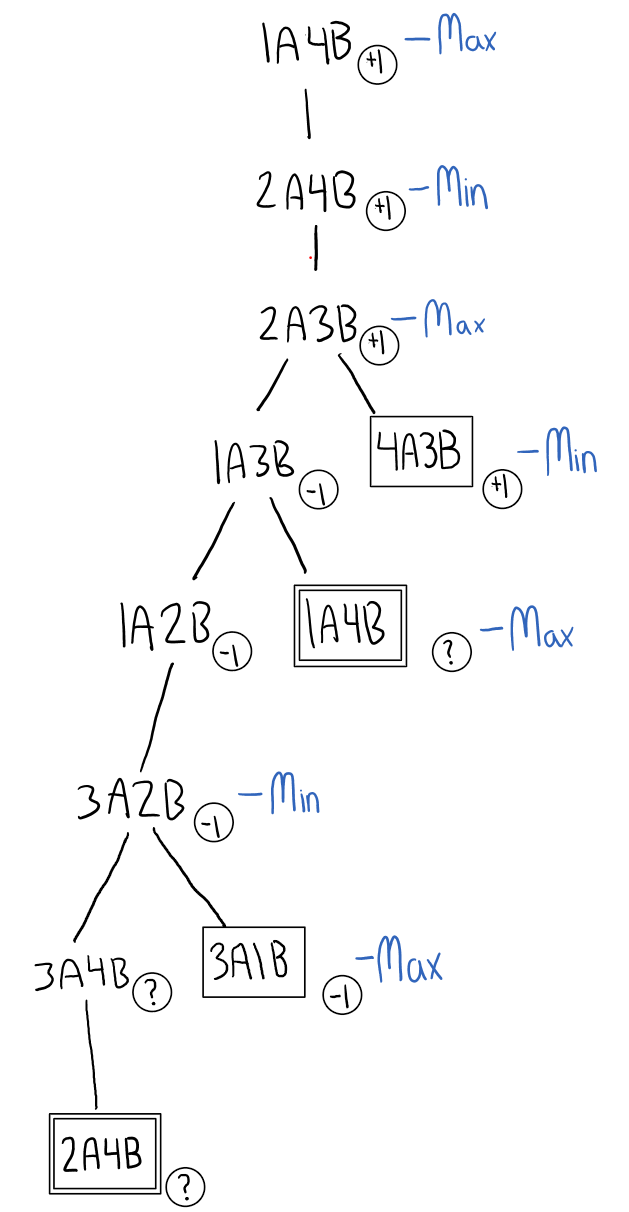
\includegraphics[scale=1]{cse545_hw2_p6_b.PNG}
			\caption{Problem 6b Adversarial Minimax.}
			\label{fig.bfs}
		\end{figure}
		\begin{verse}
			See Figure 5.
		\end{verse}
	\item Explain why the standard minimax algorithm would fail on this example and provide a method to improve the algorithm for this use case.
	\begin{verse}
		The standard minimax algorithm would never finish, as it would recurse down the and infinitely deep branch. A possible sequence of moves is A moving from 1 to 2 and back and B moving from 4 to 3 and back ad infinitum. The standard minimax algorithm would follow this infinite chain and thus never complete. There are a few ways this algorithm could be improved. One method would be to do a depth limited search that uses a heuristic evaluation, allowing the tree to only navigate down so many iterations for a decision. Since the number of states is equal to $n(n-1)$ where n is the number of boxes it is pretty easy to use a depth limit of n for an accurate evaluation. Another method, however, would be to use a dictionary to store the evaluations from one branch to be used by another. Since the state space is small with lots of repetition, we can go down one branch and get the minimax evaluations for that state and reuse them when that state is encountered again, without having to expand it. Both of these methodologies could be used for other problems with loops, given a few conditions. The first is a known methodology that would be useful in any problem with a good candidate for the depth to search down and a good heuristic for evaluating states. The latter would work in any problem where we can guarantee at least one state in an infinite sequence will be first encountered on the path to a leaf node. This would ensure that the state in the sequence would be able to return a value before entering a never-ending computation. Unfortunately this property would be hard to guarantee for a generic problem.
	\end{verse}
	\item This game can be abstracted to any n squares laid out in one dimension. Prove
			that if n is even A wins and if n is odd B wins.
	\begin{verse}
		For games with even size N A will always win as A is the first to make it to the center position, and thus has control when A and B meet. Take our base case with N=4: A moves to position 2 by necessity, B moves to position 3 by necessity, A jumps B to 4 and wins. If N is two larger, that is there is one more square until the center, A is still the first to get to the center since it is the first to move. B can choose to hold back and jump A when it gets closer, but because A can move first the furthest location B could theoretically wait is one position from the center. That is, A moves to center and then moves one more space, only to be jumped by B. This would put A and B equal distant from their respective goals, with B at the center square on A's side and A on the center square on B's side. A, however, moves first, and thus can reach its goal first so long as it never doubles back, giving it a guaranteed victory.
	\end{verse}
	\begin{verse}
		For games with odd size N, the opposite is true and B will always in. Take the base case where N = 3. A moves to position 2 and is then jumped by B from position 1 to position 3, allowing B to win. With an odd size N, there is only one center square which A, as the first to move is guaranteed to reach first. Since A and B are equidistant from the squares adjacent to the center, B will be in the adjacent square and can now jump A making it one square closer to its goal than A. Despite A moving first, B will now reach its goal first. If A doesn't choose to move into the center position, it will have to move back one position and let B move into the center. A can now move back to the position adjacent to the center, but will be jumped by B which is even closer to its goal. The further A holds towards its own end the closer B will be to its goal relative to A when one finally does jump the other. Thus B can always win if it plays optimally.
	\end{verse}
\end{enumerate}
\end{problem}
\begin{problem}{7}
	Programming Assignment - Write Alpha-Beta Pruning Algorithm.
	\begin{verse}
		See alpha\_beta.py file for implementation.
	\end{verse}
\end{problem}
\end{document}
